\subsection{Setup}

\subsubsection{Datasets}

All the input files we used are in the format of edges among nodes making it straightforward to parse them as showed in Figure \ref{fig:graphfileformat}. We opted to use this format instead of parsing the graph as an adjacency list, since this approach allows us to make the parsing in parallel in Map-Reduce in a straightforward way. Essentially, each mapper task will take as input a part of the whole graph and produce the corresponding output for that part.

\begin{verbbox}
node_from_1 node_to_1
node_from_2 node_to_2
...
node_from_n node_to_n
\end{verbbox}

\begin{figure}[ht]
  \centering
  \theverbbox
  \caption{Graph file format}
  \label{fig:graphfileformat}
\end{figure}

We used different graph files taken from Stanford's Large Network Dataset Collection \cite{datasets} which is an open-source repository of graphs with varying sizes to measure both the Sequential and Map-Redude algorithm performance. This repository contains a lot of different graphs which describe real-world data (social networks, web-pages/links) and range from a few hundred to millions or even billions of nodes and edges. The following table describes different metrics of each one:

\begin{table}[h!]
\begin{center}
\begin{tabular}{|c|c|c|}
\hline
{\bf Name} & {\bf Nodes}& {\bf Edges} \\
\hline
\hline
simple\_graph   & 10  & 14  \\
\hline
medium\_graph   & 534  & 9626 \\
\hline
ego-Facebook   & 4039  & 88234 \\
\hline
ego-Gplus   & 107614  & 13673453 \\
\hline
big\_graph   & 19670319  & 146213222 \\
\hline
\end{tabular}
\caption{Graphs}
\label{tb:graphfiles}
\end{center}
\end{table}

\subsubsection{Infrastructure}

We used an r3.xlarge to run the sequential algorithm for the different types of graphs we had in our disposal. For the Map-Reduce algorithms we used a relatively small cluster of 1 master (m3.large) and 4 slave machines (r3.xlarge) using a custom script that adds some bootstrap actions to increase the amount of memory assigned to each task as well as change the time when the reducers start to get executed based on the completion ratio of the mapper tasks. All these machines were hosted in AWS services.


\subsection{Sequential}
We used an implementation of Tarjan's Algorithm that has $O(|V| + |E|)$ worst case performance. It uses a Depth-First-Approach (DFS) as described in Section \ref{sec:algo}. It begins at an arbitrary node and  visits every node of the graph exactly once. As it is going through the graph it will be generating the various connected components.

\begin{table}[!h]
\scriptsize
\begin{center}
\begin{tabular}{|c|c|c|c|}
\hline
{\bf Graph} & {\bf Parse (ms)} & {\bf Compute (ms)} & {\bf components \#} \\
\hline
\hline
simple\_graph   & 4  & 0.247 & 3 \\
\hline
medium\_graph   & 98  & 3 & 2 \\
\hline
ego-Facebook   & 232 & 14 & 1325  \\
\hline
ego-Gplus   & 49497 & 1104 & 37249 \\
\hline
big\_graph   & ?  & ? & ?  \\
\hline
\end{tabular}
\caption{Sequential times}
\label{tb:sequentialtimes}
\end{center}
\end{table}

The results here are as expected. The algorithm performs really well when using small files and the total execution time is really small. However, we can see that as the files grow bigger and bigger the parsing time starts becoming the dominating factor that takes up most of the total execution time. The big graph instance was not successfully run on a single machine because of an out-of-memory error. The next step is to try with a really big virtual machine in AWS with enough memory that can handle it.

\subsection{Map-Reduce}

\subsubsection{Hash-to-Min}

Table \ref{tb:MapReducetimes} contains the execution time for the Map-Reduce implementation for each input graph file. We can see that using Map-Reduce for really small files is not very efficient but the real advantage is when using it to process large files. Specifically,  using Map-Reduce we were able to process the big\_graph file which failed on a single machine due to memory limitations.

\begin{table}[h!]
\footnotesize
\begin{center}
\begin{tabular}{|c|c|c|}
\hline
{\bf Graph} & {\bf Phase 1 (sec)} & {\bf Phase 2 (sec)}\\
\hline
\hline
simple\_graph   & 23  & 82 \\
\hline
medium\_graph   & 25 & 115 \\
\hline
ego-Facebook   & 25 & 180 \\
\hline
ego-Gplus   & 67  & 193 \\
\hline
big\_graph   & 153 & 1840 \\
\hline
\end{tabular}
\caption{Map-Reduce times}
\label{tb:MapReducetimes}
\end{center}
\end{table}

Figure \ref{fig:mapreduce_graph} shows an overview of the times it took us to run the Map-Reduce jobs for the different graphs. It is obvious that the parsing time now is linear to the size of input since it is being split among the multiple mappers. This is one advantage of Map-Reduce. We can also observe that using Map-Reduce for small graphs is more of an actual overhead rather than helpful. However, when it comes to large graphs Map-Reduce performs really well and it is possible to even parse the big graph successfully. The pattern here suggests that even when the graph becomes bigger we can see that the actually running time for the algorithm is linear to the input (counting nodes and edges together). For example, the big graph is 12 times bigger than the ego Gplus graph and the running time is around 10 times more.

\begin{figure}[!h]
 \centering
    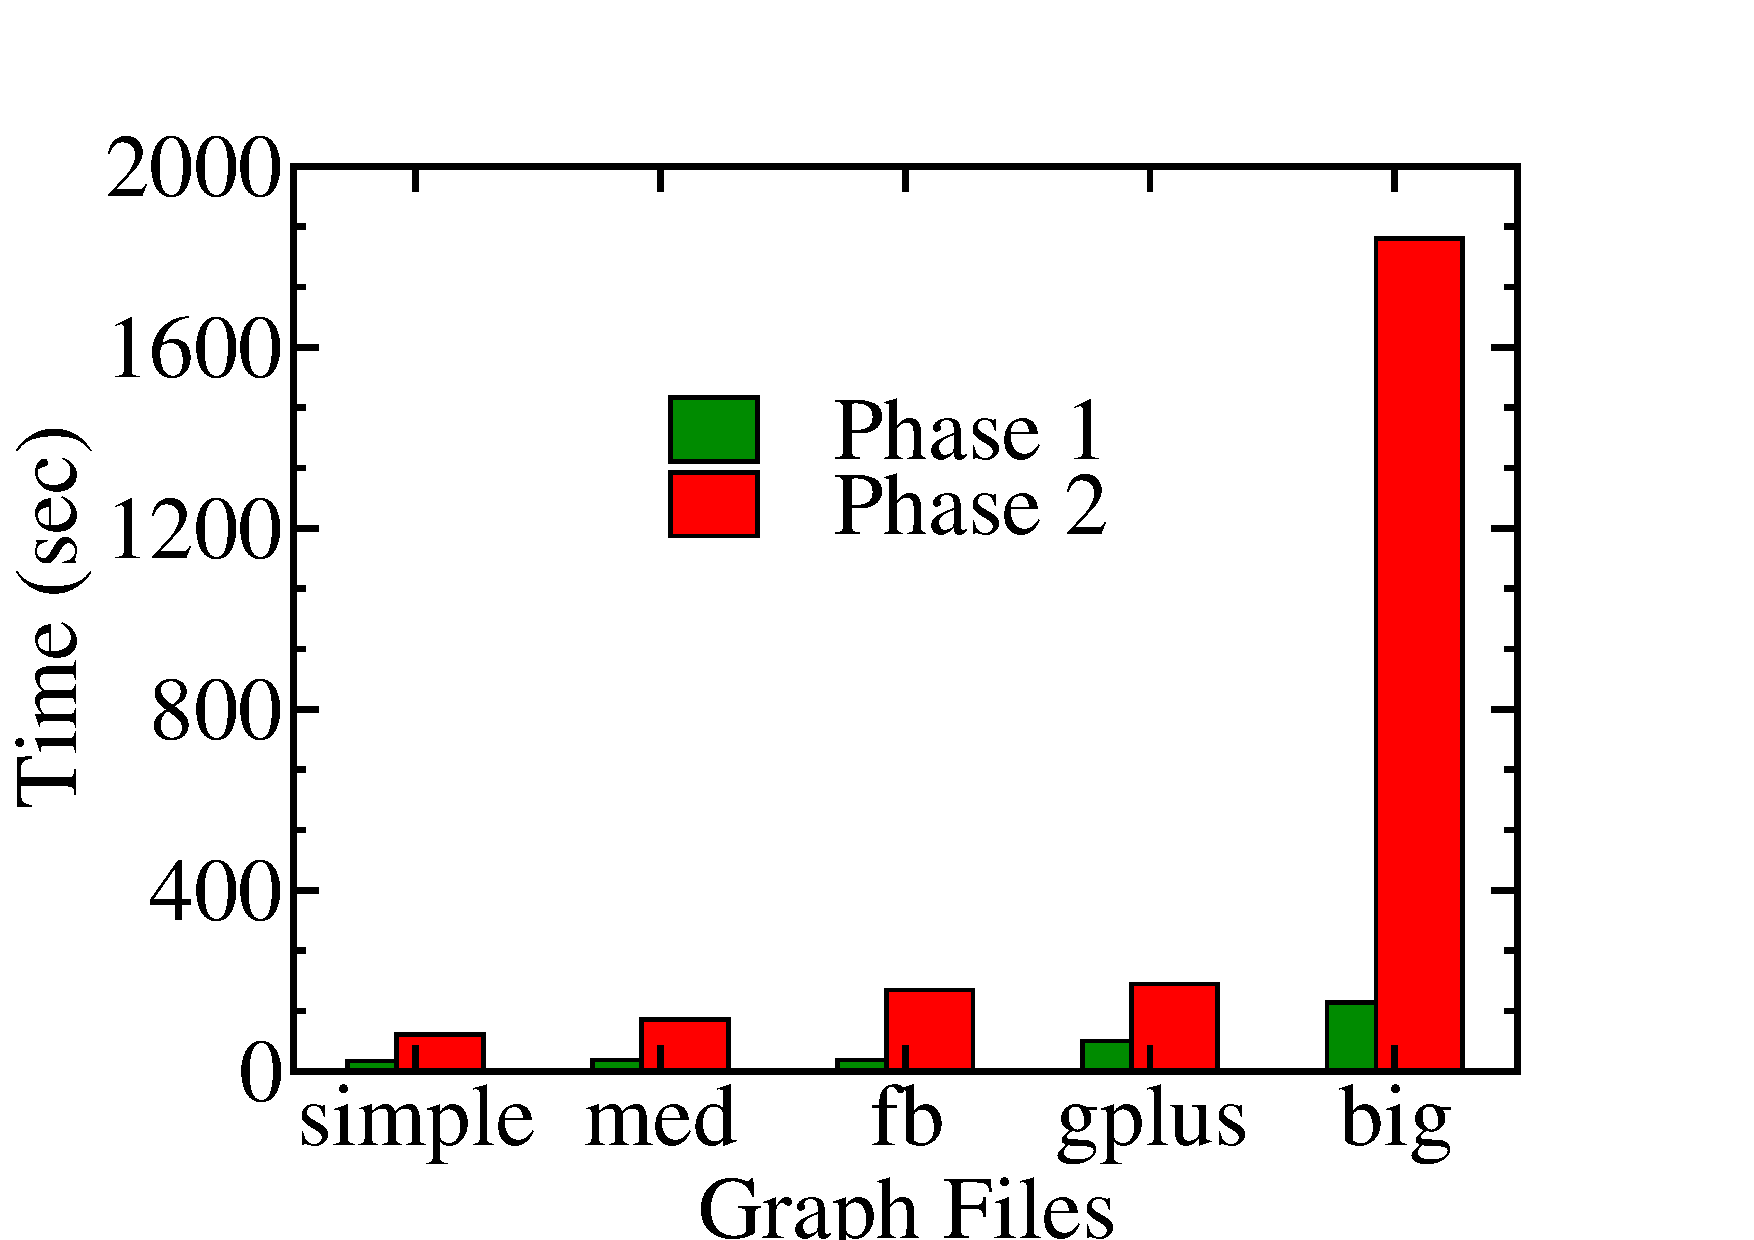
\includegraphics[width=15pc]{figures/mapreduce_graph}
	\caption{Map-Reduce running times}
    \label{fig:mapreduce_graph}
\end{figure}

We also used the Ganglia monitoring tool available on Amazon AWS EMR service. Using Ganglia we could monitor our cluster and export multiple metrics regarding CPU usage, memory usage and identify possible bottlenecks of our algorithm. Figure \ref{fig:cpu_usage} shows the CPU utilization of one slave node, while running the Hash-to-Min algorithm for the big graph. As we can see, the CPU utilization hits 100\% during some peaks, while falling lower during other intervals (possibly during initialization/termination of mapper or reducer tasks).

\begin{figure}[!h]
 \centering
    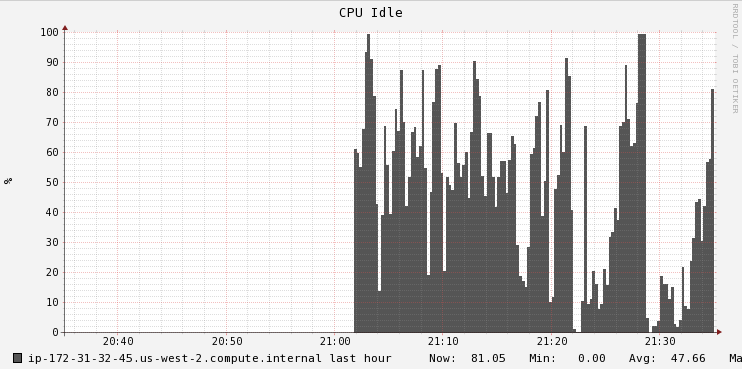
\includegraphics[width=15pc]{figures/cpu_usage}
	\caption{CPU utilization of one slave node}
    \label{fig:cpu_usage}
\end{figure}

Other useful information we can retrieve from Ganglia includes the memory usage of the JVM processes running on our cluster. As discussed before, Hash-to-Min requires a fair amount of main memory, since it tries to construct a cluster of nodes in one reducer. If there is a very big connected component, then the memory requirements for this reducer task can become quite large. Figure \ref{fig:memory_usage} presents the memory usage of one slave node. As we can see , while the program is running the memory requirements are significant for each JVM process running on the node.

\begin{figure}[!h]
 \centering
    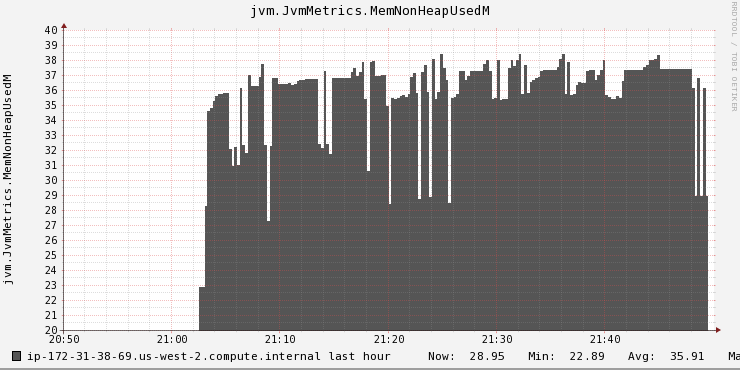
\includegraphics[width=15pc]{figures/memory_usage}
	\caption{Memory usage of one slave node}
    \label{fig:memory_usage}
\end{figure}

\subsubsection{Two-Phase}

Two-Phase algorithm proved to be more complicated to implement than Hash-to-Min. The main difficulty of this algorithm is to implement the correct convergence criteria so it stops executing after it has completed calculating the connected components. In order to check this, one needs to check if the output of a previous operation (large star or small star) has changed in regards to the current operation. This requires to check the output files of the reduce step and compare them. There are a couple of caveats in doing this. If we try to compare the files in the driver function, this defeats the purpose of running the program on Map-Reduce since it will slow down the whole process (the output file are comparable to the initial graph in size). Another approach that we tried to follow, is to get the md5 checksum of the files and compare them with the ones from the previous step. Although this worked for the smallest graph we had available (simple\_graph) which was completed successfully within a similar time limit as the Hash-to-Min algorithm, it didn't successfully apply on the other graphs. Essentially, the algorithm didn't converge inside its theoretical limits and was dragged in an infinite loop of repeating steps. We experimented by trying different approaches (\eg we took into account the original graph file on top of the previous step) but they were still stuck in the same convergence problem. It is also possible that the check for the checksums which are provided by Amazon's S3 service automatically has a fault, depending on the exact algorithm they use to calculate them. Thus, it may not be safe to use them as a stop condition and other approaches might need to be considered (see Section \ref{sec:conclusion}).
